\documentclass{beamer}
\usepackage{hyperref}
%% \usepackage[CJKmath=true, AutoFakeBold = true]{xeCJK}
\usepackage[T1]{fontenc}
%% \setCJKmainfont{AR PL KaitiM GB} % Set Chinese font to KaiTi (calligraphy style)

% Other packages
\usepackage{latexsym,xcolor,multicol,booktabs,calligra}
\usepackage{amssymb,amsfonts,amsmath,amsthm,mathrsfs,mathptmx} % Common math packages
\usepackage{graphicx,pstricks,listings,stackengine}
\usefonttheme[onlymath]{serif} % Use serif font for equations (better appearance)

% Other packages (new)
% \usepackage{latexsym,amsmath,xcolor,multicol,booktabs,calligra} % math symbols, equations, colors, columns, tables, and calligraphic font
\usepackage[linesnumbered,ruled,vlined]{algorithm2e}
\SetKwComment{Comment}{$\triangleright$ }{} % The argument will be surrounded by /* ... */
\SetAlCapFnt{\footnotesize} % Make caption text smaller
\SetAlCapNameFnt{\footnotesize} % Make "Algorithm" label smaller
\usepackage{graphicx} % Enables inclusion and scaling of images (\includegraphics)
\usepackage{animate} % Provides support for frame-by-frame animations (\animategraphics)
\usepackage{subcaption} % Provides support for subfigures (subfigure environment with captions)
\usepackage{fontawesome5} % Provides scalable vector icons (Font Awesome 5 icons)

\captionsetup{
    skip=5pt, % Space between figure and caption
    belowskip=0pt % Space below the caption (reduces gap after caption)
}

\newcommand{\source}[1]{\par\footnotesize Source: #1} % Defines a reusable command to display the image/table source in small font below the caption

\renewcommand{\today}{\number\year-\number\month-\number\day}
\renewcommand{\alert}[1]{\textbf{\color{swufe}#1}}

% Title page setup
% \author{Lu** \inst{1}, Zhang** \inst{1}}
\author[Topics]{Topics}

\title[Title of Presentation]{Title of Presentation}
% \subtitle{Jiangnan University Academic Report Beamer Template}
%% \institute[JNU]{\normalsize{\inst{1} School of Business \quad Jiangnan University \quad \textit{****@qq.com}}}
\institute[Session 1]{
    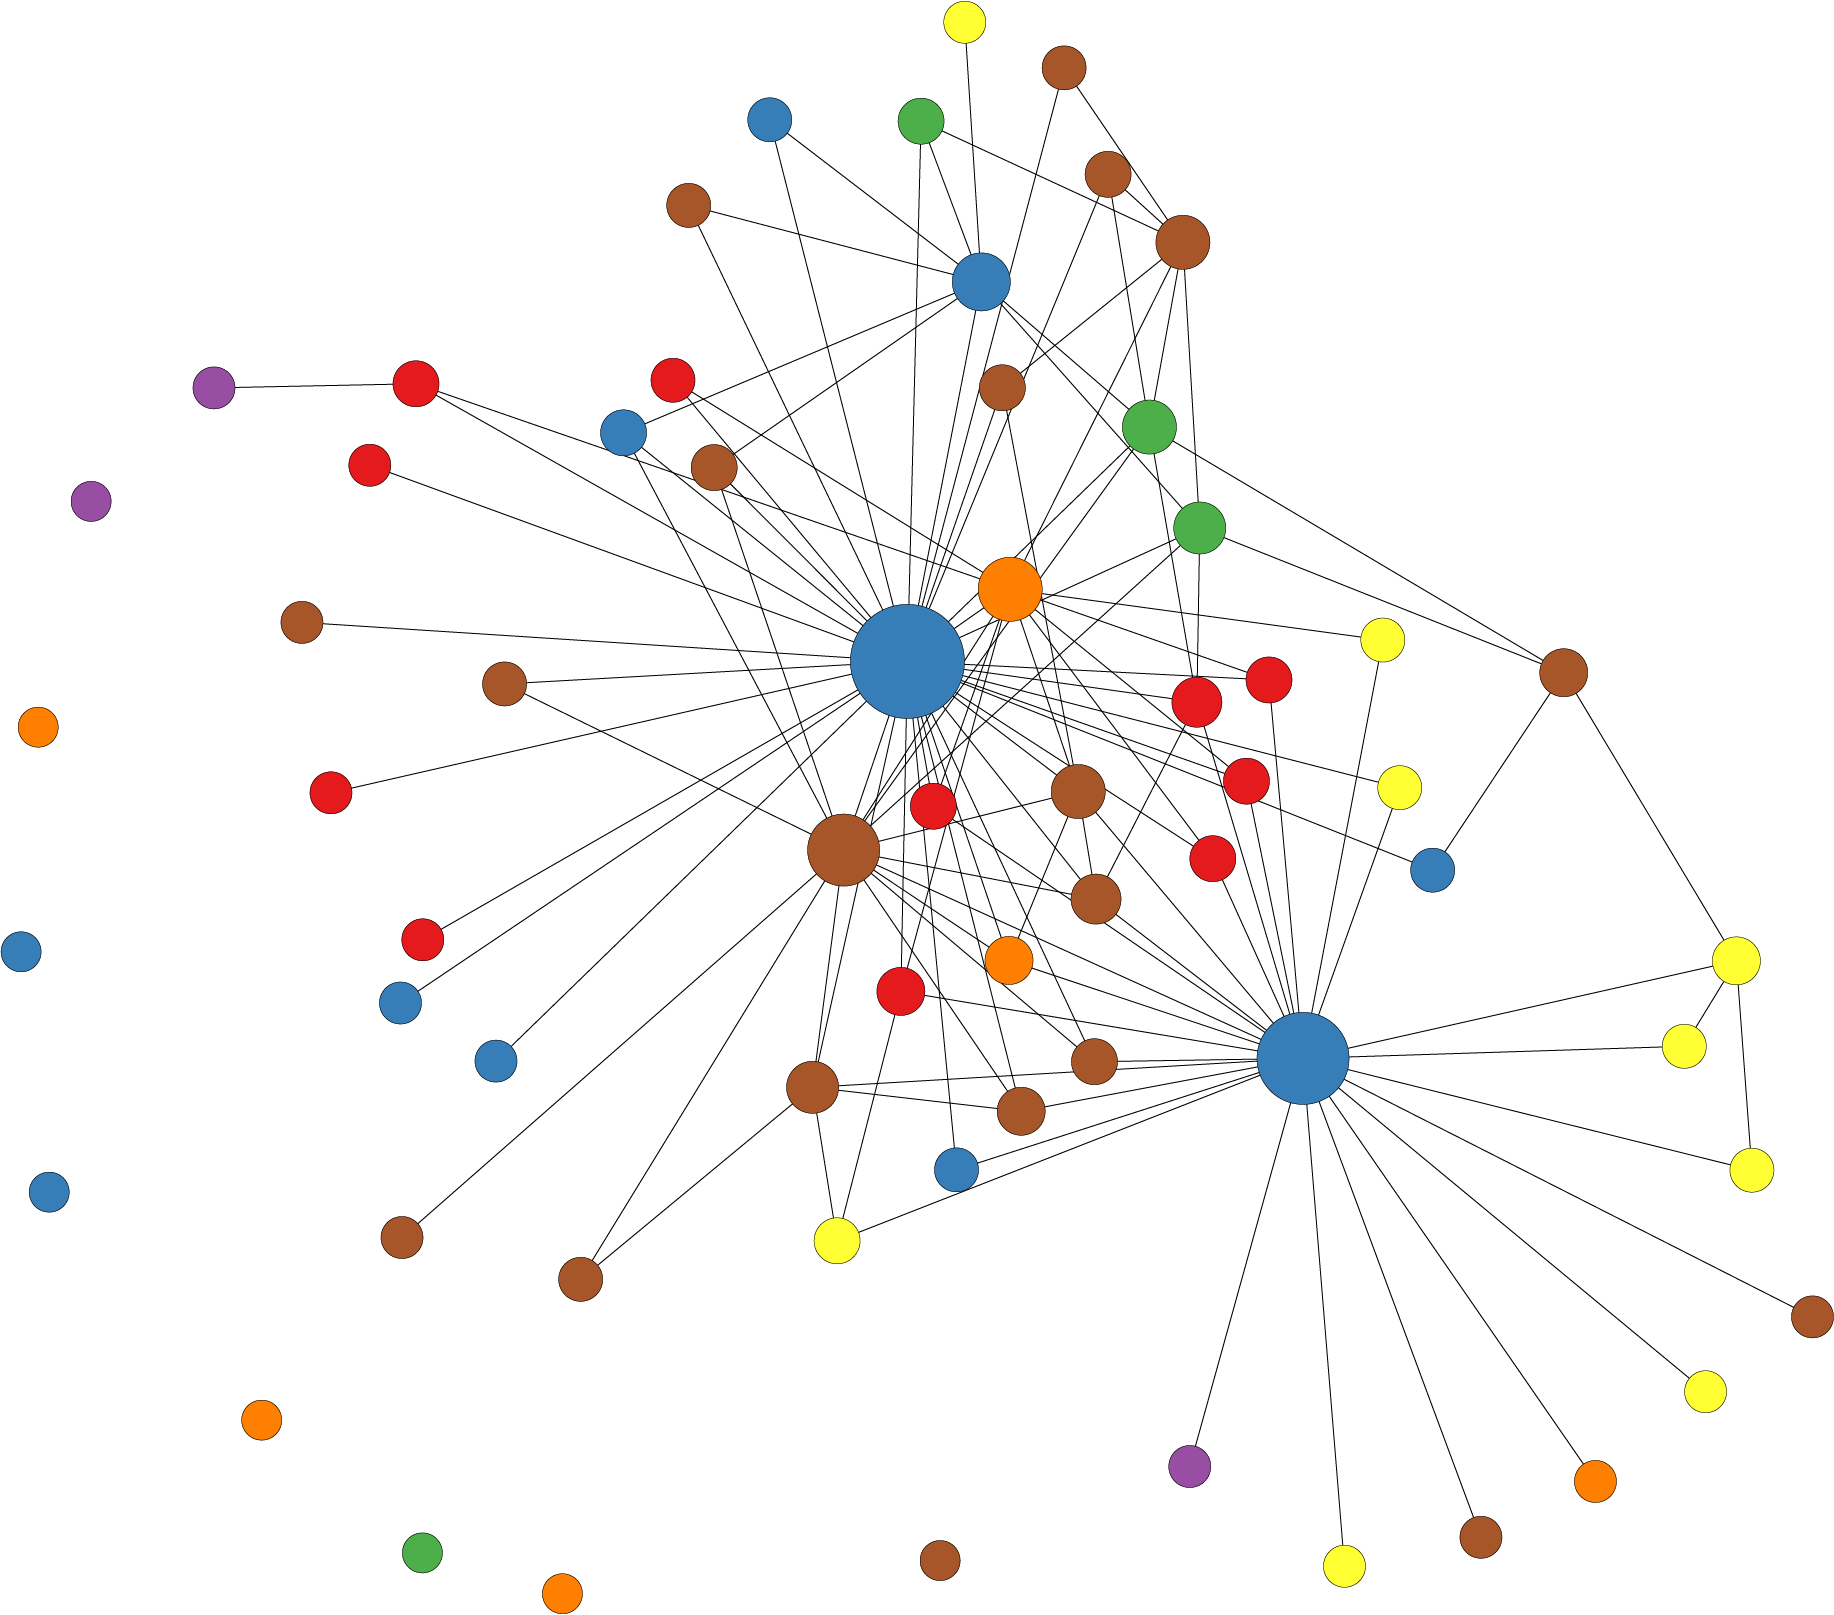
\includegraphics[width=0.3\linewidth]{pic/logo_graph.png}
}

% \date{\today}
\date{\scriptsize March, 2026}

\usepackage{JNU}

% Defs
\def\cmd#1{\texttt{\color[RGB]{0, 0, 139}\footnotesize $\backslash$#1}}
\def\env#1{\texttt{\color[RGB]{0, 0, 139}\footnotesize #1}}

\lstset{
    language=[LaTeX]TeX,
    basicstyle=\ttfamily\footnotesize,
    keywordstyle=\bfseries\color[RGB]{0, 0, 139},
    stringstyle=\color[RGB]{50, 50, 50},
    numbers=left,
    numberstyle=\small\color{gray},
    rulesepcolor=\color{red!20!green!20!blue!20},
    frame=shadowbox,
}

\begin{document}

\begin{frame}
    \titlepage
    \begin{figure}[htpb]
        \begin{center}
            %% 
\includegraphics[width=0.55\linewidth]{pic/jiangnan_logo.png}
        \end{center}
    \end{figure}
\end{frame}

\begin{frame}
    \tableofcontents
\end{frame}

\section{Introduction}
    \begin{frame}{Blocks}
        \begin{block}{Info}
            General content
        \end{block}

        \begin{alertblock}{Warning}
            Important message
        \end{alertblock}

        \begin{exampleblock}{Example}
            Example content
        \end{exampleblock}

        \begin{note}
            {Write your notes here}
        \end{note}
    \end{frame}

    \begin{frame}{Basic}
        In mathematics and computer science, a graph (network) is defined as $G = (V, E)$, where $V = \{v_1, v_2, ..., v_{n}\}$ is the nodes (or \textit{vertices}, or \textit{points}) set and $E = \{e_1, e_2, ..., e_{m}\}, e_i \in V \times V$ a set of edges (or \textit{lines}, or \textit{arcs}) formed by unordered pairs of nodes. \\

        \scriptsize Number of nodes is denoted $|V|$. \\
        Number of edges is denoted $|E|$.

        \begin{figure}[htp!]
            \centering
            
\includegraphics[
                width=0.3\linewidth,
                trim=0pt 0pt 0pt 0pt, % trim: left bottom right top
                clip
            ]{pic/default_image.png}
            \caption{My image.}
            \source{Author, 2024.}
            % \label{fig:my_image}
        \end{figure}

        \begin{note}
            {Introduce your self}
        \end{note}
    \end{frame}

    \begin{frame}{Basic}
        \begin{alertblock}{Adjacency matrix}
            Adjacency matrix \textbf{$A$}, is an $n \times n$ matrix where: 
            \[
                A_{i, j} =
                \begin{cases}
                1 & \text{if there is an edge from vertex } i \text{ to vertex } j \\
                0 & \text{otherwise}
                \end{cases}
            \]
        \end{alertblock}

        \begin{figure}
            \centering
            \begin{subfigure}{0.2\textwidth}
                \centering
                
\includegraphics[
                    width=\linewidth,
                    trim=0pt 0pt 0pt 0pt, % trim: left bottom right top
                    clip
                ]{pic/default_image.png}
                \caption{My image.}
                % \source{Author, 2024.}
            \end{subfigure}
            % \hfill
            \hspace{1cm}
            \begin{subfigure}{0.2\textwidth}
                \centering
                
\includegraphics[
                    width=\linewidth,
                    trim=0pt 0pt 0pt 0pt, % trim: left bottom right top
                    clip
                ]{pic/default_image.png}
                \caption{My image.}
                % \source{Author, 2024.}
            \end{subfigure}

            \caption{My image.}
            \source{Author, 2024.}
            % \label{fig:my_image}
        \end{figure}

        \begin{note}
            {Write your notes here}
        \end{note}
    \end{frame}

    \begin{frame}{Basic}
        \begin{alertblock}{Idea}
            Does the shortest path from $a$ to $c$ go through $b$?
        \end{alertblock}

        \begin{figure}[htp!]
            \centering
            
\includegraphics[
                width=0.3\linewidth,
                trim=0pt 0pt 0pt 0pt, % trim: left bottom right top
                clip
            ]{pic/default_image.png}
            \caption{My image.}
            \source{Author, 2024.}
            % \label{fig:my_image}
        \end{figure}

        \begin{note}
            {Introduce your self}
        \end{note}
    \end{frame}

    \begin{frame}{Basic}
        BFS is a graph traversal algorithm that explores nodes level by level, visiting all nodes at a given distance from the starting node before moving to the next level. \newline

        Description:
        \begin{itemize}
            \item Uses a queue (FIFO) to manage the nodes to be explored.
            \item Marks visited nodes to avoid cycles or repeated visits.
            \item Ideal for finding the shortest path in unweighted graphs.
        \end{itemize}

        \begin{note}
            {Introduce your self}
        \end{note}
    \end{frame}

\section{Methodology}
    \begin{frame}{Equations}
        Furthermore, each edge $e \in E$ is said to join two vertices. If $e$ joins $u, v \in V$, then $e = (u, v)$. Vertices $u$ and $v$ are said to be adjacent. \\
        
        \begin{alertblock}{Neighborhood}
            \begin{equation}
                N(v) = \{w \in V ∣ v \neq w \land (v, w) \in E\}
                % \label{eq:equation1}
            \end{equation}
        \end{alertblock}

        \begin{note}
            {Introduce your self}
        \end{note}
    \end{frame}

    \begin{frame}{Equations}
        \begin{alertblock}{Unnumbered equation}
            \begin{equation*}
                J(\theta) = \mathbb{E}_{\pi_\theta}[G_t]
                % \label{eq:equation1}
            \end{equation*}
        \end{alertblock}

        \begin{alertblock}{Multi-line equations}
            \begin{align}
                Q_{\mathrm{target}} &= r + \gamma Q^\pi(s', \pi_\theta(s') + \epsilon)\\
                \epsilon &\sim \mathrm{clip}(\mathcal{N}(0, \sigma), -c, c)
                % \label{eq:equation1}
            \end{align}
        \end{alertblock}
    \end{frame}

    \begin{frame}
        \begin{alertblock}{Equation with numbers}
            % Taken from Mathmode.tex
            \begin{multline}
                A=\lim_{n\rightarrow\infty}\Delta x\left(a^{2}+\left(a^{2}+2a\Delta x+\left(\Delta x\right)^{2}\right)\right.\label{eq:reset}\\
                +\left(a^{2}+2\cdot2a\Delta x+2^{2}\left(\Delta x\right)^{2}\right)\\
                +\left(a^{2}+2\cdot3a\Delta x+3^{2}\left(\Delta x\right)^{2}\right)\\
                +\ldots\\
                \left.+\left(a^{2}+2\cdot(n-1)a\Delta x+(n-1)^{2}\left(\Delta x\right)^{2}\right)\right)\\
                =\frac{1}{3}\left(b^{3}-a^{3}\right)
                % \label{eq:equation1}
            \end{multline}
        \end{alertblock}
    \end{frame}

    \begin{frame}{Algorithms}
        \begin{algorithm}[H]
            \scriptsize
            % \footnotesize
            \DontPrintSemicolon
            % \SetAlgoLined
            % \SetNoline
            
            \SetKwInOut{Input}{Input}
            \SetKwInOut{Output}{Output}
            
            \Input{$G$, $s$ \Comment*[r]{Graph $G$ and a source node $s$}}
            \Output{All nodes reachable from $s$}
            
            % \BlankLine
            $Q \gets \varnothing$ \Comment*[r]{Create an empty queue}
            $V \gets \varnothing$ \Comment*[r]{Create an empty set of visited}
            $enqueue(Q, s)$\;
            $append(V, s)$\;
            
            \While{$Q \neq \varnothing$}{
                $v \gets dequeue(Q)$\;
                $print(v)$\;

                \ForEach{$u \in N(v)$}{ % \Comment*[r]{process all neighbors of node $u$}
                    \If{$u \notin V$}{
                        $append(V, u)$\;
                        $enqueue(Q, u)$
                    }
                }
            }
            % \Return max\;
            \caption{My algorithm.}
            % \label{tab:algorithm}
        \end{algorithm}
        
        \begin{note}
            {Introduce your self}
        \end{note}
    \end{frame}

    \begin{frame}{Two columns}
        \begin{columns}[t] % The "c" centered vertical alignment, "t" top vertical alignment
            \begin{column}{0.45\textwidth}
                \begin{itemize}
                    \item \textbf{Graph traversal}
                    \begin{itemize}
                        \item Breadth-First Search
                        \item Depth-First Search
                    \end{itemize}
                \end{itemize}
            \end{column}
            
            \begin{column}{0.55\textwidth}
                \begin{itemize}
                    \item \textbf{Shortest path algorithms}
                    \begin{itemize}
                        \item Dijkstra
                        \item Floyd–Warshall
                        \item Bellman-Ford
                    \end{itemize}
                \end{itemize}
            \end{column}
        \end{columns}

        \begin{note}
            {Introduce your self}
        \end{note}
    \end{frame}

    \begin{frame}{Two columns}        
        \begin{columns}[t] % The "c" option specifies centered vertical alignment while the "t" option is used for top vertical alignment
            \begin{column}{0.6\textwidth}
                \begin{enumerate}
                    \item Visit the adjacent unvisited node. Mark as visited, display, and insert (queue) in a queue.
                    \item In case no adjacent node is found, remove the first node from the queue.
                    \item Repeat steps 1, and 2 until the queue is empty.
                \end{enumerate}
            \end{column}
            
            \begin{column}{0.4\textwidth}
                \begin{figure}[htp!]
                    \centering
                    
\includegraphics[
                        width=0.6\linewidth,
                        trim=0pt 0pt 0pt 0pt, % trim: left bottom right top
                        clip
                    ]{pic/default_image.png}
                    \caption{My image.}
                    \source{Author, 2024.}
                    % \label{fig:my_image}
                \end{figure}
            \end{column}
        \end{columns}
        
        \begin{note}
            {Introduce your self}
        \end{note}
    \end{frame}

    \begin{frame}{Lists}
        \begin{itemize}
            \item Install requirements
                \begin{itemize}
                    \item \texttt{Python}
                    \item \texttt{Numpy}
                    \item \texttt{Pandas}
                    \item \texttt{NetworkX}
                    \item \texttt{Matplotlib}
                \end{itemize}
            \item Topics 
                \begin{itemize}
                    \item Create graphs
                    \item Graphs visualization
                \end{itemize}
            \item Lab
                \begin{itemize}
                    \item \href{https://drive.google.com/file/d/1e3h6VeZp3ocwF68VzBbgxJJbF98NSzZT/view?usp=sharing}{
                            \beamergotobutton{\faGoogle\ Open in Google Colab}
                        }
                \end{itemize}
        \end{itemize}

        \begin{note}
            {Write your notes here}
        \end{note}
    \end{frame}

    \begin{frame}{Sequential list display}
        \begin{itemize}[<+-| alert@+>]
            \item Many people use \LaTeX{}, and many universities have their own Beamer themes
            \item For Chinese support, use Xe\LaTeX{} as the compiler
        \end{itemize}

        \begin{note}
            {Introduce your self}
        \end{note}
    \end{frame}

    \begin{frame}[allowframebreaks]{Lists (dynamic)}
        \begin{itemize}
            \setlength{\itemsep}{10pt}
            \item This template is modified from a Tsinghua University project
            \item Original template: \url{https://www.overleaf.com/latex/templates/thu-beamer-theme/vwnqmzndvwyb}
            \item Minor modifications were made
            \item Style adjusted to personal preference
            \item Added small Beamer usage examples
            \item Replaced default fonts with more readable ones
            \item Fixed inconsistent Chinese font issues
            \item Changed math fonts to serif for better appearance
            \item \alert{Use \cmd{alert} to emphasize text}
            \item This template is modified from a Tsinghua University project
            \item Original template: \url{https://www.overleaf.com/latex/templates/thu-beamer-theme/vwnqmzndvwyb}
        \end{itemize}

        \begin{note}
            {Introduce your self}
        \end{note}
    \end{frame}

\section{Results}
    \begin{frame}{Table}
        \begin{table}[htp!]
            \centering
            \caption{My table.}
            % \label{tab:table1}
            \begin{tabular}{ll}\toprule
                Representation & Complexity \\\midrule
                Adjacency matrix & $O(|V|^2)$ \\
                Adjacency list & $O(|V| + |E|)$ \\
                Edge list & $O(|E|)$  \\
                Incidence matrix & $O(|V||E|)$  \\\bottomrule
            \end{tabular}
        \end{table}

        \begin{note}
            {Write your notes here}
        \end{note}
    \end{frame}

    \begin{frame}{Table (custom)}
        \begin{table}[htp!]
            \scriptsize
            \centering
            \caption{My table.}
            % \label{tab:table1}
            \begin{tabular}{p{2.2cm}p{4cm}p{4cm}}\toprule
                Representation & Advantages & Disadvantages \\\midrule
                Adjacency matrix & Simple structure, constant-time edge lookup. & High memory usage for large sparse graphs. \\
                Adjacency list & Memory efficient for sparse graphs, easy to iterate over neighbors. & Edge existence check may be slower. \\
                Edge list & Very simple representation, useful for algorithms that process edges sequentially. & Inefficient for neighbor queries.  \\
                Incidence matrix & Useful in some theoretical formulations and algebraic graph analysis. & High memory usage and rarely used in practical implementations. \\\bottomrule
            \end{tabular}
        \end{table}

        \begin{note}
            {Write your notes here}
        \end{note}
    \end{frame}

    \begin{frame}{Figure}
        \begin{figure}[htp!]
            \centering
            
\includegraphics[
                width=0.3\linewidth,
                trim=0pt 0pt 0pt 0pt, % trim: left bottom right top
                clip
            ]{pic/default_image.png}
            \caption{My image.}
            \source{Author, 2024.}
            % \label{fig:my_image}
        \end{figure}

        \begin{note}
            {Write your notes here}
        \end{note}
    \end{frame}

    \begin{frame}{Multiple figures}
        \begin{figure}
            \centering
            \begin{subfigure}{0.2\textwidth}
                \centering
                
\includegraphics[
                    width=\linewidth,
                    trim=0pt 0pt 0pt 0pt, % trim: left bottom right top
                    clip
                ]{pic/default_image.png}
                \caption{My image.}
                % \source{Author, 2024.}
            \end{subfigure}
            \hfill
            \begin{subfigure}{0.2\textwidth}
                \centering
                
\includegraphics[
                    width=\linewidth,
                    trim=0pt 0pt 0pt 0pt, % trim: left bottom right top
                    clip
                ]{pic/default_image.png}
                \caption{My image.}
                % \source{Author, 2024.}
            \end{subfigure}
            \hfill
            \begin{subfigure}{0.2\textwidth}
                \centering
                
\includegraphics[
                    width=\linewidth,
                    trim=0pt 0pt 0pt 0pt, % trim: left bottom right top
                    clip
                ]{pic/default_image.png}
                \caption{My image.}
                % \source{Author, 2024.}
            \end{subfigure}
            \hfill
            \begin{subfigure}{0.2\textwidth}
                \centering
                
\includegraphics[
                    width=\linewidth,
                    trim=0pt 0pt 0pt 0pt, % trim: left bottom right top
                    clip
                ]{pic/default_image.png}
                \caption{My image.}
                % \source{Author, 2024.}
            \end{subfigure}

            \caption{My image.}
            \source{Author, 2024.}
            % \label{fig:my_image}
        \end{figure}

        \begin{note}
            {Write your notes here}
        \end{note}
    \end{frame}

    \begin{frame}{Figure (dynamic)}
        \begin{figure}
            \centering
            \animategraphics[width=\textwidth,loop,autoplay]
            {5} % frame rate
            {pic/imd/freiburg_matches-} % path to figures
            {0} % start index
            {15} % end index
            \caption{My image.}
            \source{Author, 2024.}
            % \label{fig:my_image}
        \end{figure}

        \begin{note}
            {Write your notes here}
        \end{note}
    \end{frame}

\section*{References}
    \begin{frame}
        \begin{center}
            {\Huge\calligra Thanks!} \\
            % {\Huge\textit{Thank you for your attention!}}\\
            {\Huge $\infty$} \\
            % edwin.alvarez@pucp.edu.pe\\
            % \url{https://github.com/win7}
        \end{center}
    \end{frame}
    
    %========================
    % bibliography
    %========================
    % \input{ref.bib}
    \begin{frame}[allowframebreaks]
        \footnotesize % use this command to resize
        % \bibliography{ref}
        % \bibliographystyle{unsrt}
        % \bibliographystyle{alpha}
        
        \begin{itemize}
            \item Erciyes, K. (2018). \textit{Guide to graph algorithms} % (pp. 15-35). Springer International Publishing.
            \item Yao Ma, Jiliang Tang. (2021). \textit{Deep Learning on Graphs}.
            \item Stamile C., Marzullo A., Deusebio E. (2021). \textit{Graph Machine Learning}.
            \item Wu, L., Cui, P., Pei, J., Zhao, L., \& Guo, X. (2022). \textit{Graph neural networks: foundation, frontiers and applications}. % In Proceedings of the 28th ACM SIGKDD conference on knowledge discovery and data mining (pp. 4840-4841).            
            % \item Knickerbocker D. (2023). \textit{Graph Network Science with Python}.
            \item Knickerbocker, D. (2023). \textit{Network Science with Python}. % Packt Publishing Ltd.
            \item Labonne, M. (2023). \textit{Hands-On Graph Neural Networks Using Python}.
            \item Broadwater, K., \& Stillman, N. (2025). \textit{Graph neural networks in action}. % Simon and Schuster.
        \end{itemize}
    \end{frame}

\end{document}
